%% Should originally belong to \subsection{Working Demo}.
%% Moving it here to move the image up a page.
\begin{figure*}[hbt!]
\centering
%%%%%%%%%%%%%%%%%%%%%%%%%%%%%%%%%%%%%
\begin{subfigure}[b]{.4\textwidth}
\begin{lstlisting}[basicstyle=\scriptsize\sffamily, stepnumber=1, numbers=left, numbersep=-6pt, framexleftmargin=0mm, framexrightmargin=0mm, language=Java, emph={allGames}]
    List<Game> allGames = gameMapper.getAllGamesByLeague(league);
    for (Game game : allGames) {
        game.getTeam1().setGame(game);
        game.getTeam2().setGame(game);
    }
    Collections.sort(allGames, new GameComparator());
\end{lstlisting}
%\caption{A listing}
\end{subfigure}
%%%%%%%%%%%%%%%%%%%%%%%%%%%%%%%%%%%%%%%%%%%%
\begin{subfigure}[b]{.4\textwidth}
\begin{lstlisting}[basicstyle=\scriptsize\sffamily, stepnumber=1, numbers=left, numbersep=-6pt, framexleftmargin=0mm, framexrightmargin=0mm, language=java, emph={annotationVersion}]
    private boolean isValidUntil(Until annotation) {
        if (annotation != null) {
            double annotationVersion = annotation.value();
            if (annotationVersion <= version) {
                return false;
            }
        }
        return true;
    }
\end{lstlisting}
\end{subfigure}
%%%%%%%%%%%%%%%%%%%%%%%%%%%%%%%%%%%%%%%%%%%%
\begin{subfigure}[b]{.45\textwidth}
  \centering
  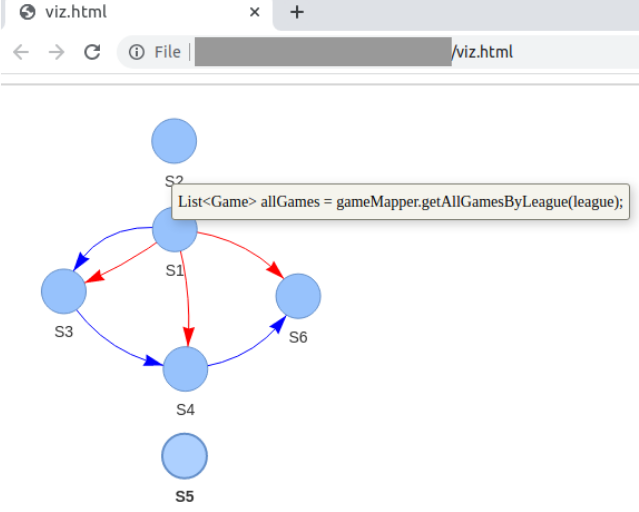
\includegraphics[width=0.7\linewidth]{icse23-demo-figures/lst-partial2.png}
  \vspace{0.75cm}
\end{subfigure}
%%%%%%%%%%%%%%%%%%%%%%%%%%%%%%%%%%%%%%%%%%%%
\begin{subfigure}[b]{.45\textwidth}
  \centering
  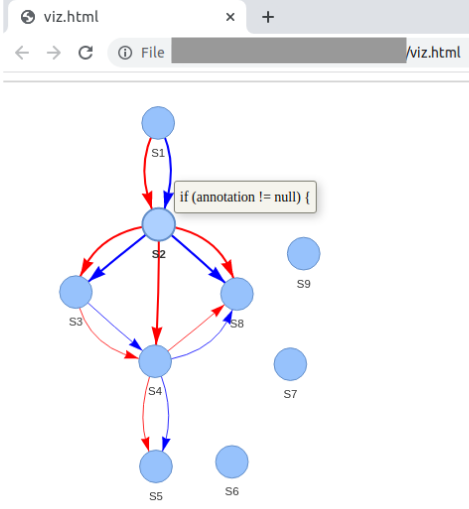
\includegraphics[width=0.7\linewidth]{icse23-demo-figures/lst-complete2.png}
\end{subfigure}
%%%%%%%%%%%%%%%%%%%%%%%%%%%%%%%%%%%%%%%%%%%%
\caption{Partial (top-left) and complete (top-right) Java code listings and their CFG/PDGs output by \tool (bottom).}
\label{fig:demo}
\end{figure*}

\section{Getting Started with \tool}
\subsection{Environment Setup}
\tool was implemented as a Python package using 
several libraries including \code{pytorch}, \code{transformers}, \code{pyvis},
etc. A working environment can be set up with the help of 
\code{conda} package manager in the Anaconda Python distribution~\cite{anaconda}, 
and the provided YAML configuration file with the following 
command: \code{\$ conda env create -f environment.yml}

\subsection{Usage}
The prototype for \tool can be run in the virtual environment as a command-line utility as follows:

\noindent \code{\$ python infer.py -i <input-path> -o <output-format>}
\begin{itemize}
    \item \code{-i}: Path to a \code{.txt} file containing the code snippet, or a directory containing multiple input \code{.txt} files. 
    \item \code{-o \{json|html\}}: \code{json} option outputs a JSON file containing predicted CFG/PDG edge information between the statements in the code snippet(s). \code{html} option draws an interactive directed graph bearing CFG (\textit{blue}) and PDG (\textit{red}) edges, further saving it as an HTML file(s). 
\end{itemize}

After loading the pre-trained dependency inference model, \tool takes a blazing quick 
%\textcolor{red}{0.\_\_} seconds on an Intel 8\textsuperscript{th} generation CPU and is even faster on a machine with a GPU ($\sim$0.02 seconds with an Nvidia Quadro P4000 GPU).
$\sim$0.02 seconds on a machine with an Nvidia Quadro P4000 GPU.

\subsection{Working Demo}
In Figure~\ref{fig:demo}, we illustrate a working demonstration of \tool. At the top, we present two Java code snippets: partial (left), and complete (right). The corresponding CFG/PDGs drawn by \tool are drawn at the bottom. The control-flow edges and program dependence edges are highlighted in \textit{blue} and \textit{red} colors respectively. Clicking on a node bolds all edges coming to, or leaving the node. In addition, hovering over a node lists the corresponding statement in a text box.

In the partial code snippet (left), statement-block $S_3$--$S_4$ iterates over the variable \code{allGames} defined in statement $S_1$. Due to the loop dependence, program (data)-dependence edges $S_1{\rightarrow}S_3$ and $S_1{\rightarrow}S_4$ are identified (left-bottom). Besides, a \textit{def-use} chain and consequently, a data-dependence edge $S_1{\rightarrow}S_6$  over the identifier \code{allGames} is also identified.

For the complete code snippet (right), all control-flow edges are predicted accurately. In addition, \tool predicts all but one control-dependence edge, that from $S_2{\rightarrow}S_7$. However, given that it correctly identifies the control-flow edge between $S_2$ and $S_7$, it is likely that it was not able to conclude whether $S_2$ determines the execution of $S_7$, resulting in the miss.

Statements such as "\code{\{}" or "\code{\}}" are not syntactic statements, and do not share a dependence relation with other statements in the code snippet. Thus, our tool draws them as free nodes $S_5$ (left-bottom); $S_6$, $S_7$, and $S_9$ (right-bottom) in the graphs.

\subsection{Tool Availability}
All code and data used to build and run \tool is available at {https://github.com/deeppda-icse23/DeepPDA}. Also, our video demo can be found at \textcolor{red}{{Add.Youtube.video.link}}.